\documentclass{beamer}

\title{MAS202M Final Project}
\author{Kári Hlynsson}
\institute{University of Iceland}
\date{April 2024}

\logo{
\includegraphics[height=1.15cm]{hi_logo.pdf}\hspace{0.25cm}}
\setbeamertemplate{navigation symbols}{}
\usetheme{Singapore}

\setbeamertemplate{title page}[default][left]
\setbeamertemplate{frametitle}[default][left]

\usepackage{xcolor}
\usepackage{graphicx}
\usepackage{helvet}

\usepackage{bm}

\graphicspath{{img/}}

\definecolor{islrred}{HTML}{990000}
\definecolor{islrgreen}{HTML}{009900}
\definecolor{islrblue}{HTML}{3333b3}
\let\OldTexttt\texttt
\renewcommand{\texttt}[1]{\OldTexttt{{\textcolor{islrred}{#1}}}}

\let\OldTextit\textit
\renewcommand{\textit}[1]{\OldTextit{{\textcolor{islrgreen}{#1}}}}

\begin{document}

\begin{frame}
  \titlepage 
\end{frame}

\begin{frame}{Overview}
  \begin{itemize}
    \setlength{\itemsep}{1em}
    \item Part A: Data cleaning / clustering (30\%) 
      \begin{itemize}
        \item Removal of duplicated samples
        \item Treatment of missing values (\texttt{NA}s)
        \item Hierarchical clustering, K-means and PCA
      \end{itemize}
    \item Part B: Prediction / inference (70\%)
      \begin{itemize}
        \item \texttt{EHBP1}: LASSO and Random Forest
        \item \texttt{temp}: SVMs and KNN
      \end{itemize}
  \end{itemize}
\end{frame}

\begin{frame}
  \centering
  \Large
  \textcolor{islrblue}{Part A}
\end{frame}

\begin{frame}{Data cleaning}
  \begin{itemize}
    \item Raw data is \(1772 \times 8\), reduced to \(1672 \times 5\)
    \item The first column, \texttt{index}, was removed
    \item Covariates \texttt{col3} and \texttt{col6} were identical except
      at points where the other was \texttt{NA}. The missing observations in 
      \texttt{col3} were derived from \texttt{col6}; the latter was removed
    \item 97 observations were found to be duplicates and were removed from the
      data set
    \item 3 observations were duplicates but contained one \texttt{NA} field,
      and were not initially detected. These were also removed
    \item Following removal of duplicated, the \texttt{id} column held no
      relevant information and was subsequently removed
  \end{itemize}
\end{frame}

\begin{frame}{Data cleaning}
  \begin{itemize}
    \item The raw data contained 20 missing values
    \item Means of respective covariates was used to impute these values
  \end{itemize}
\end{frame}

\begin{frame}{Clustering}
  \begin{figure}
    \begin{center}
      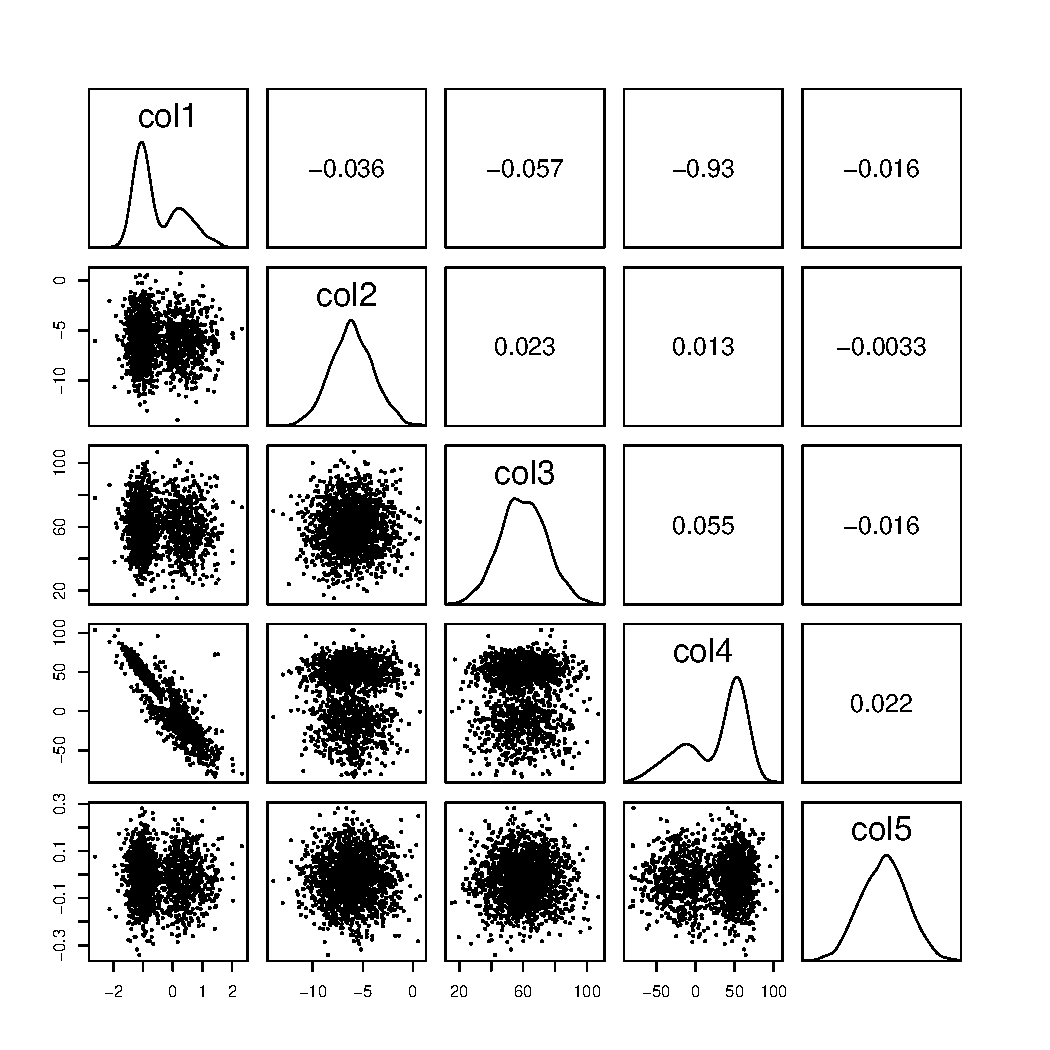
\includegraphics[width=0.7\textwidth]{pair_plot_synthetic.pdf}
    \end{center}
  \end{figure}
\end{frame}

\begin{frame}{Clustering}
  \begin{itemize}
    \item To cluster the data, hierarchical clustering and K-means were
      considered
      \begin{itemize}
        \item Each of the two methods was run on \textit{raw} and 
          \textit{scaled} data, as well as on the first two \textit{principal
          components} of the data
        \item Clustering accuracy was mainly assessed through visual 
          confirmation
      \end{itemize}
    \item Optimal clustering results were obtained for K-means clustering on
      PCA data
  \end{itemize}
\end{frame}

\begin{frame}{Clustering -- Hierarchical}
  \begin{figure}
    \begin{center}
      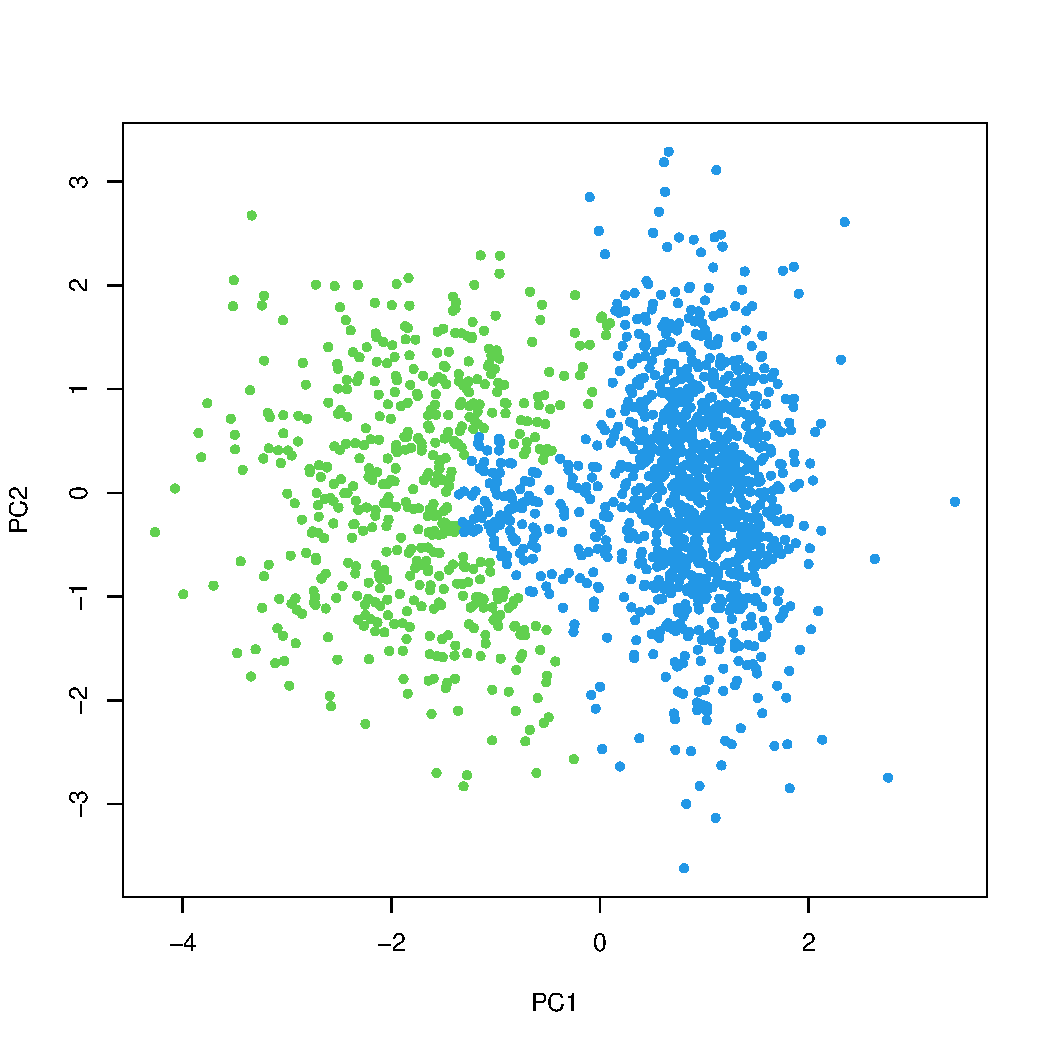
\includegraphics[width=0.7\textwidth]{hclust_pca.pdf}
    \end{center}
  \end{figure}
\end{frame}

\begin{frame}{Clustering -- K-means}
  \begin{figure}
    \begin{center}
      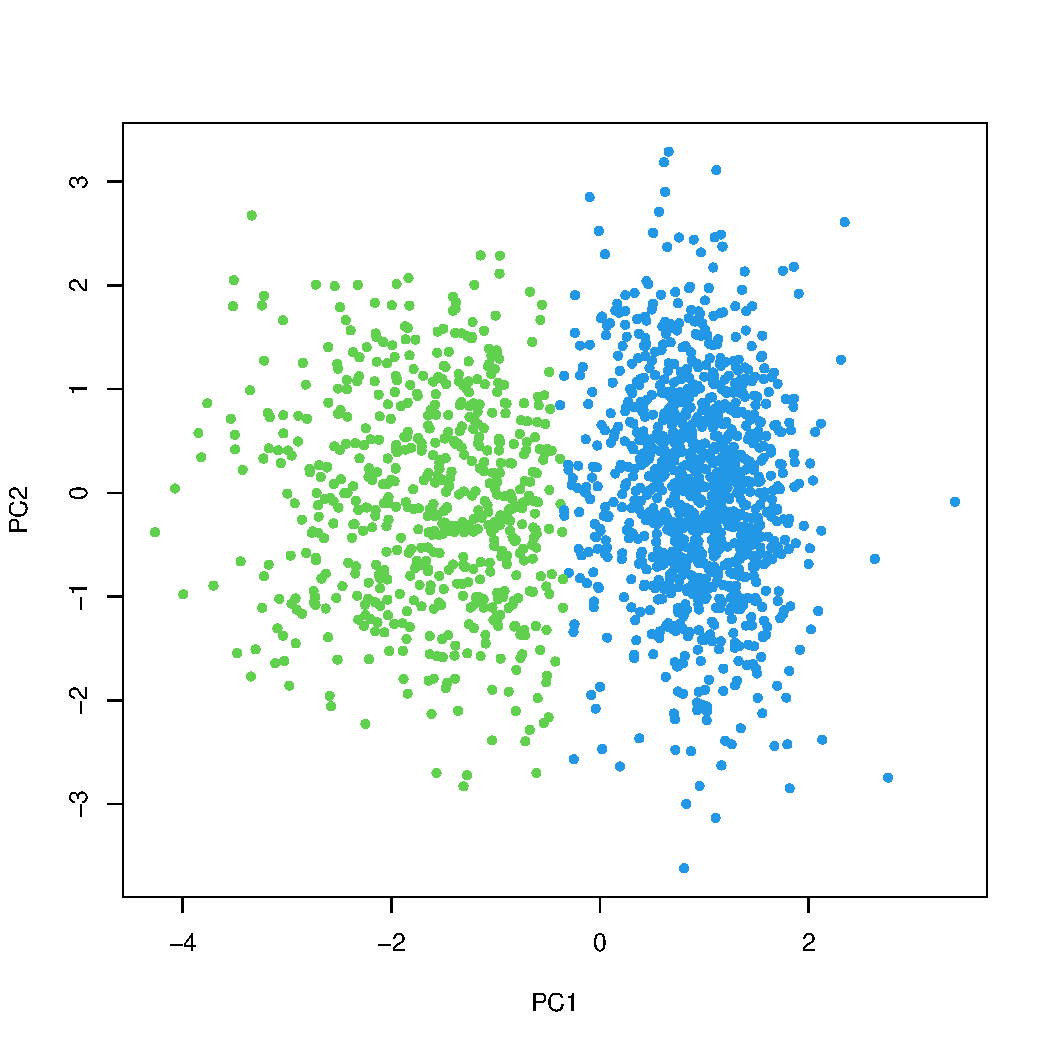
\includegraphics[width=0.7\textwidth]{knn_pca.pdf}
    \end{center}
  \end{figure}
\end{frame}


\begin{frame}
  \centering
  \Large
  \textcolor{islrblue}{Part B}
\end{frame}

\begin{frame}{Quantitative variable}
  \begin{itemize}
    \item We will consider \texttt{EHPB1}
    \item LASSO and random forest regression
  \end{itemize}
\end{frame}

\begin{frame}{LASSO}
  \begin{itemize}
    \item High dimensional setting, \(n \ll p\), motivates use
      of methods that \textit{reduce number of covariates} used in modelling
    \item LASSO was chosen for this task in the linear setting.
      Other potential candidates include ridge, PCR, PLS, AIC step
      procedures, etc.
    \item Assumes a \textit{linear relationship} between response and 
      covariates which may be overly stringent
    \item Optimise over cost hyperparameter, \(\lambda\):
      \[
        \bm\beta_{\text{LASSO}} = \underset{\bm\beta}{\text{argmin}}
        \left[\sum_{i = 1}^n (y_i - \hat y_i)^2 + \lambda \left|\sum_{j = 1}^p 
        \beta_j\right|\right]
      \]
  \end{itemize}
\end{frame}

\begin{frame}{LASSO}
  \begin{itemize}
    \item Optimal value of \(\lambda\) determined using 75\% train-test split
      using LOOCV. This gave \(\lambda \approx 0.1797\)
    \item Test set MSE \(= 0.1080\)
    \item 8 predictors were non-zero, specifying the model
      \begin{align*}
        \texttt{EHBP1} &= 0.5504 + 0.0403 \times \texttt{XIAP}
                       + 0.0826 \times \texttt{MOCS2} \\
                       &\quad + 0.4383 \times \texttt{MARS1}
                       + 0.006 \times \texttt{APPL2} \\
                       &\quad + 0.1296 \times \texttt{OPLAH}
                       + 0.071 \times \texttt{CNP} \\
                       &\quad + 0.0164 \times \texttt{RTN4IP1}
                       + 0.1734 \times \texttt{FKBP14}
      \end{align*}
  \end{itemize}
\end{frame}

\begin{frame}{LASSO}
  \begin{figure}
    \begin{center}
      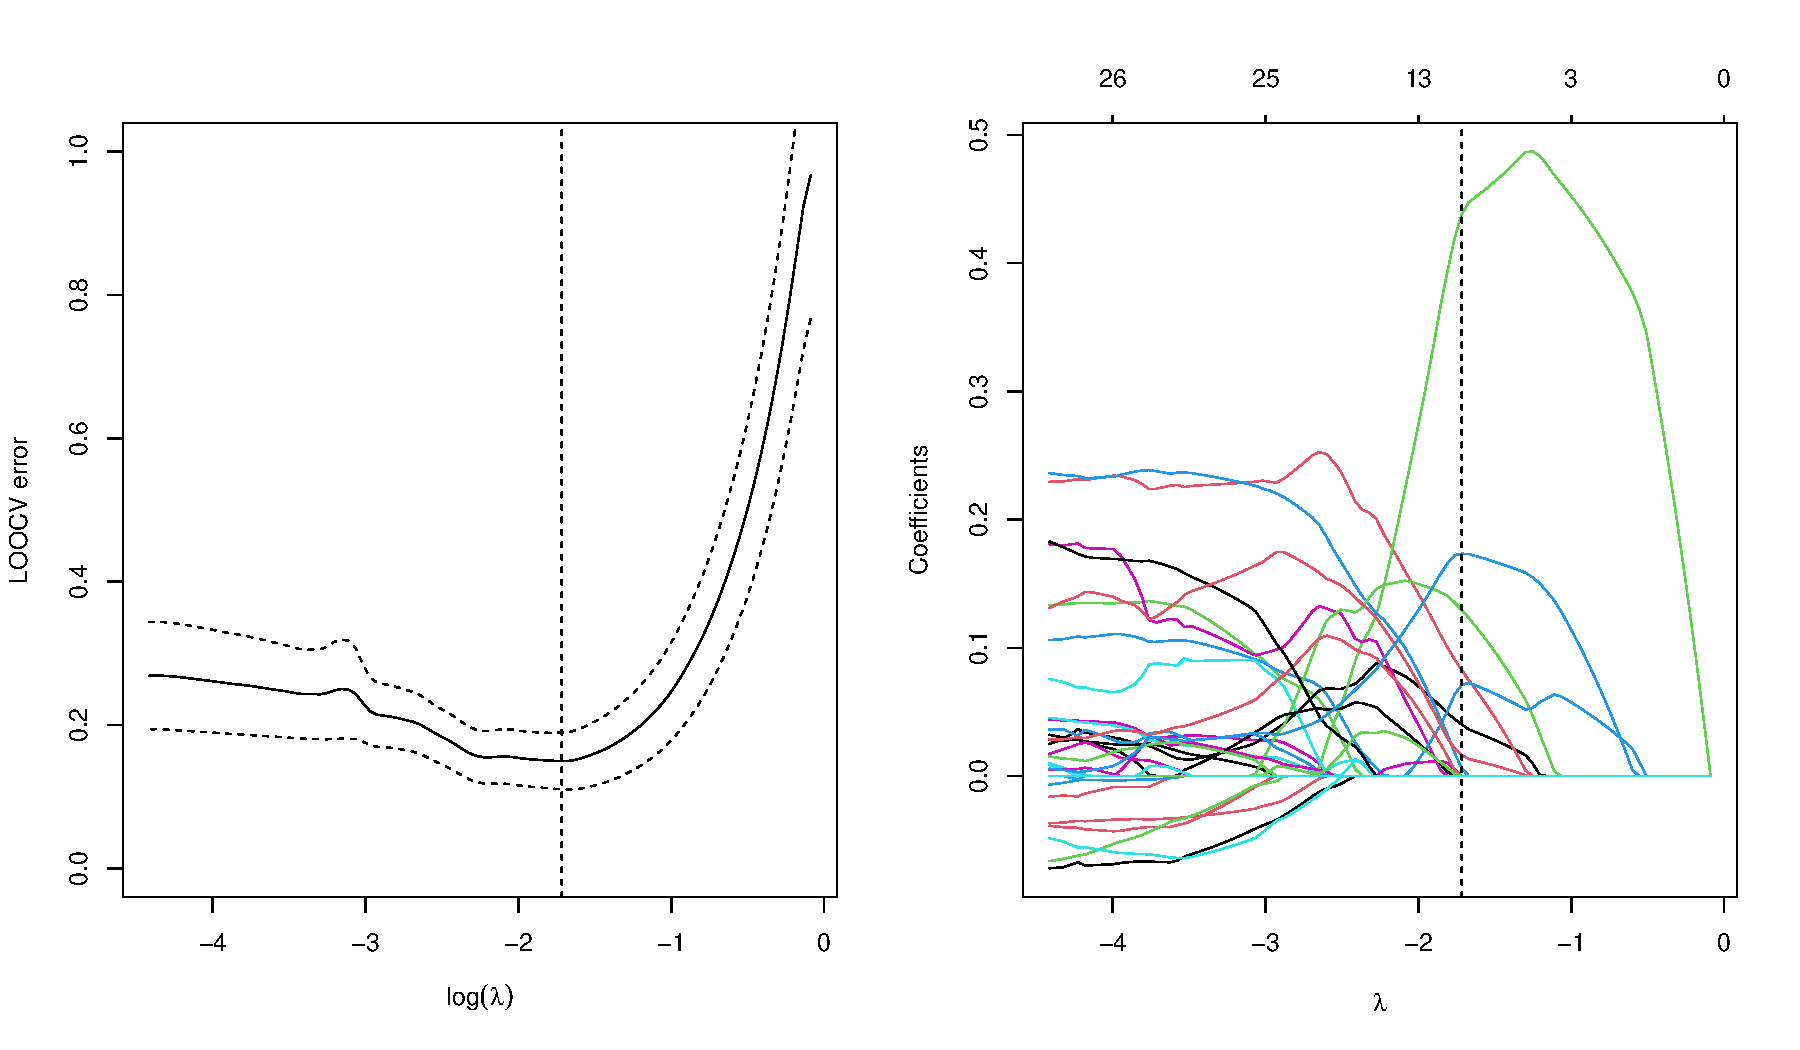
\includegraphics[width=\textwidth]{lasso_fitting.pdf}
    \end{center}
  \end{figure}
\end{frame}

\begin{frame}{LASSO}
  \begin{figure}
    \begin{center}
      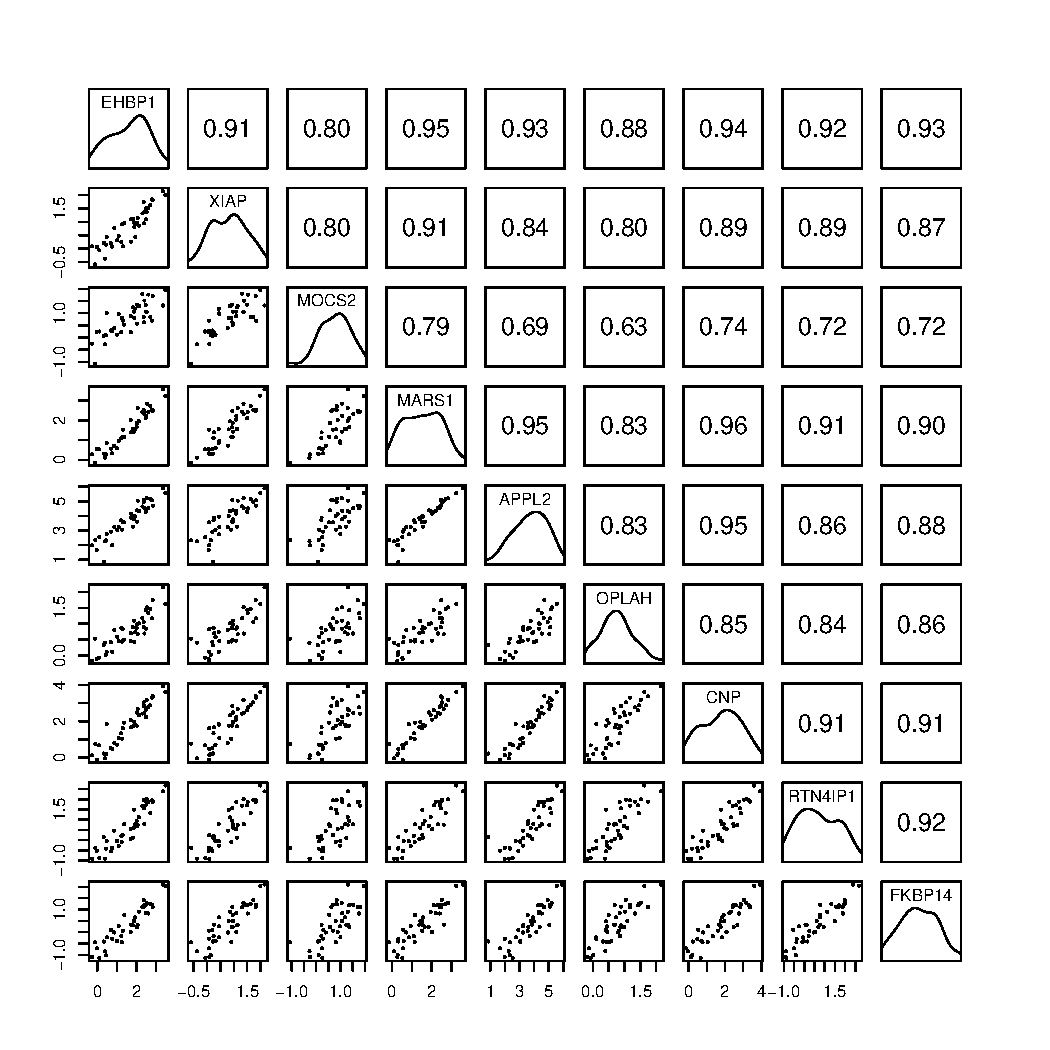
\includegraphics[width=0.7\textwidth]{lasso_nz_cov.pdf}
    \end{center}
  \end{figure}
\end{frame}

\begin{frame}{Random forest}
  \begin{itemize}
    \item Random forest regressor was tuned for optimal \texttt{mtry} with
      \texttt{ntree} = 500, yielding \texttt{mtry} = 110
    \item Works well in the \textit{high-dimensional setting} \(n \ll p\) due to 
      restricting decision trees to a \textit{subset of predictors}
    \item More \textit{candidate causal predictors} uncovered -- favourable in
      "breadth-first" scanning, e.g. for biomarkers
    \item Test set MSE of 0.1147, marginally unfavourable to LASSO.
  \end{itemize}
\end{frame}

\begin{frame}{Random forest}
 \begin{figure}
  \begin{center}
    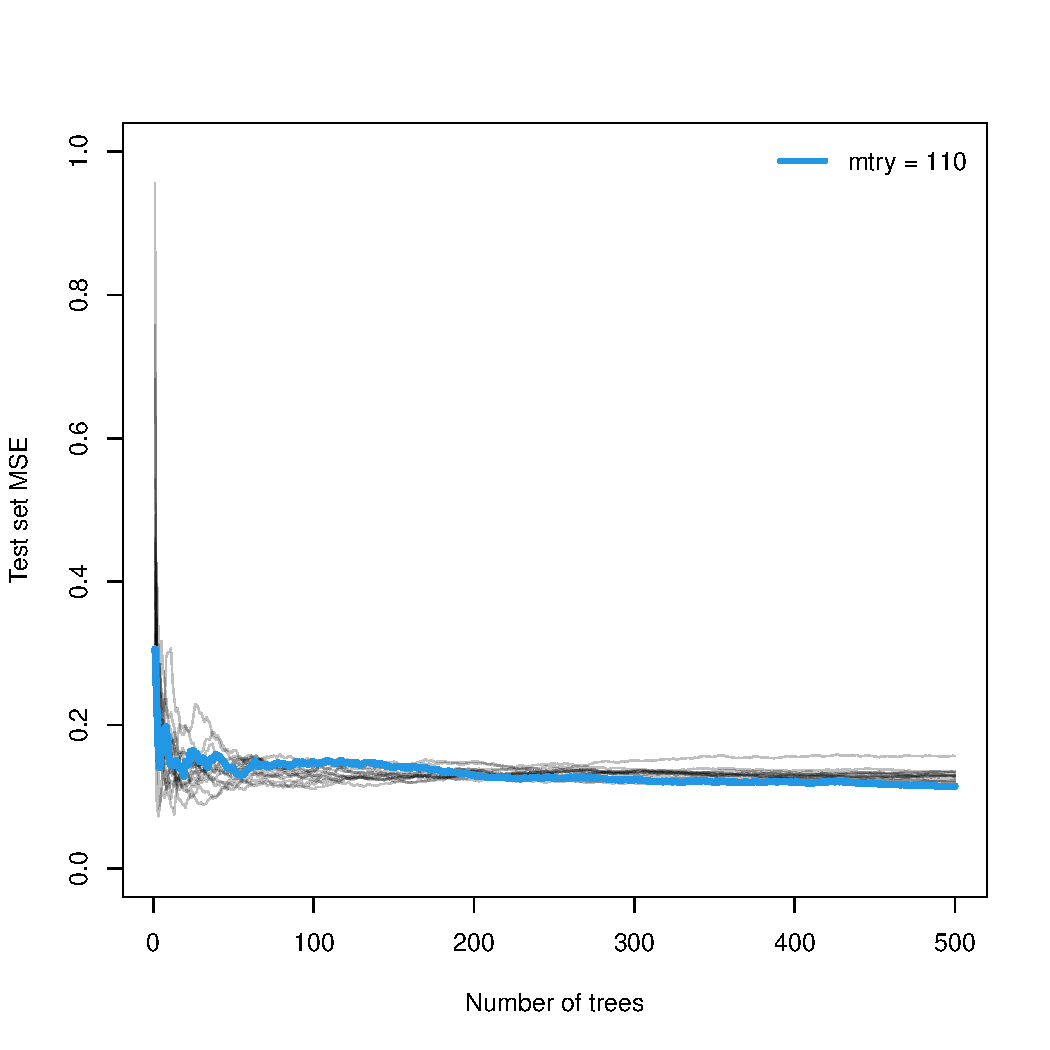
\includegraphics[width=0.7\textwidth]{rf_err.pdf}
  \end{center}
 \end{figure}
\end{frame}

\begin{frame}{Random forest}
 \begin{figure}
  \begin{center}
    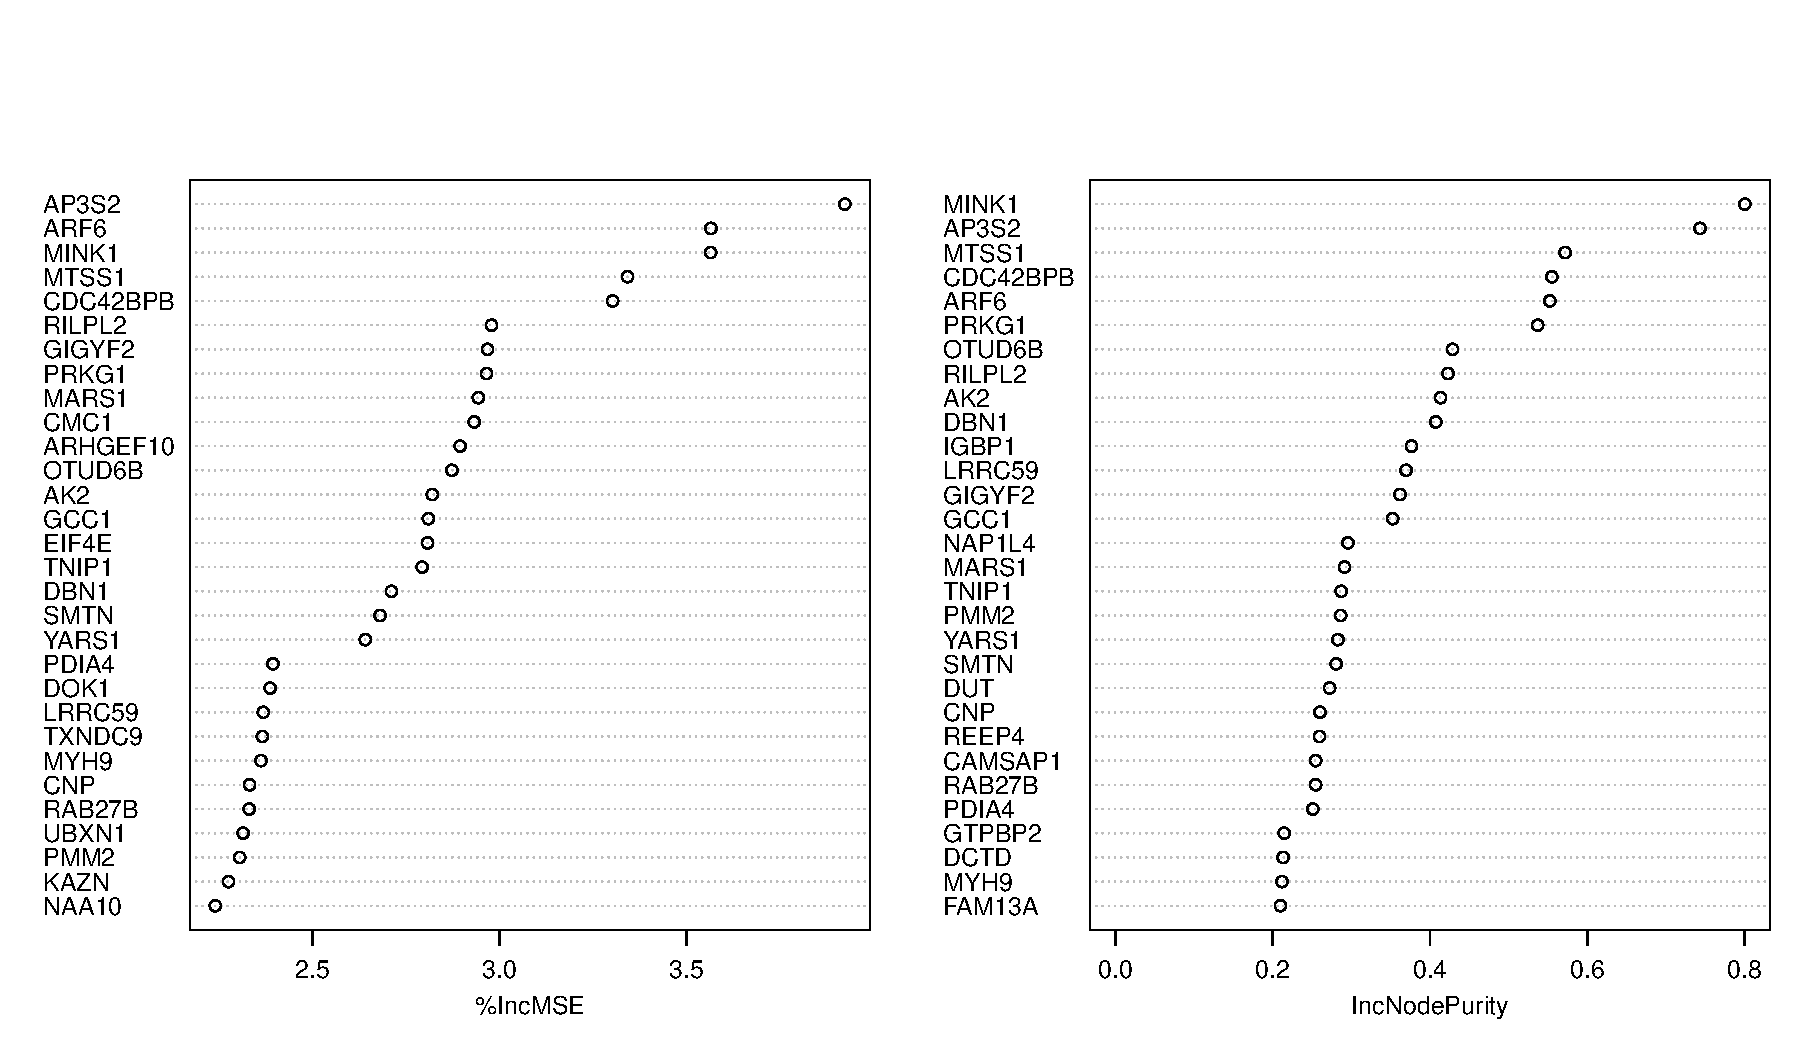
\includegraphics[width=\textwidth]{imp_plot_rf.pdf}
  \end{center}
 \end{figure}
\end{frame}

\begin{frame}{Random forest}
  \begin{figure}
    \begin{center}
      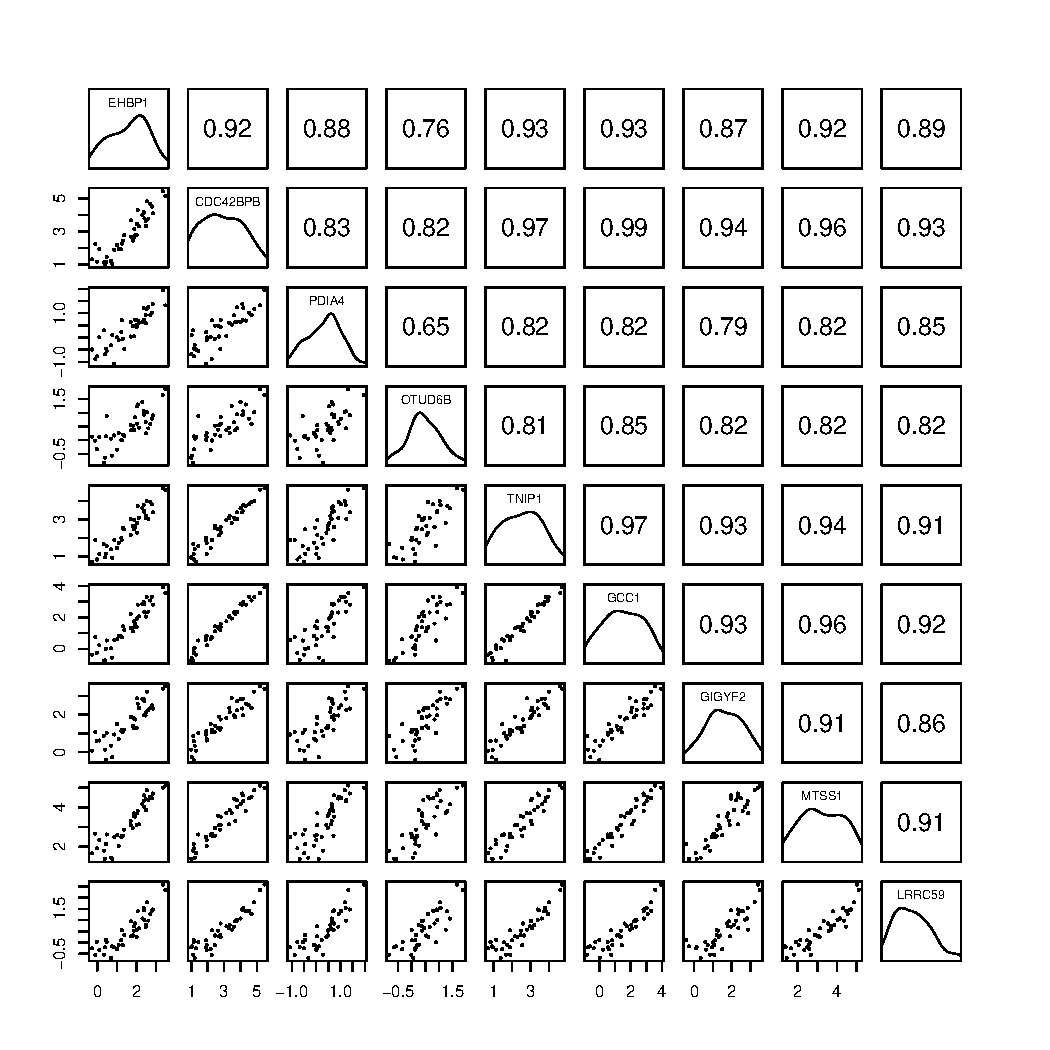
\includegraphics[width=0.7\textwidth]{rf_imp_pairs.pdf}
    \end{center}
  \end{figure}
\end{frame}

\begin{frame}{Categorical variable}
  \begin{itemize}
    \item We will study the \texttt{temp} variable 
    \item SVM and KNN
    \item Fitted on data transformed using PCA to reduce computational 
      complexity (15 components, 71.4\% var.)
  \end{itemize}
\end{frame}

\begin{frame}{Categorical variable}
  \begin{figure}
    \begin{center}
      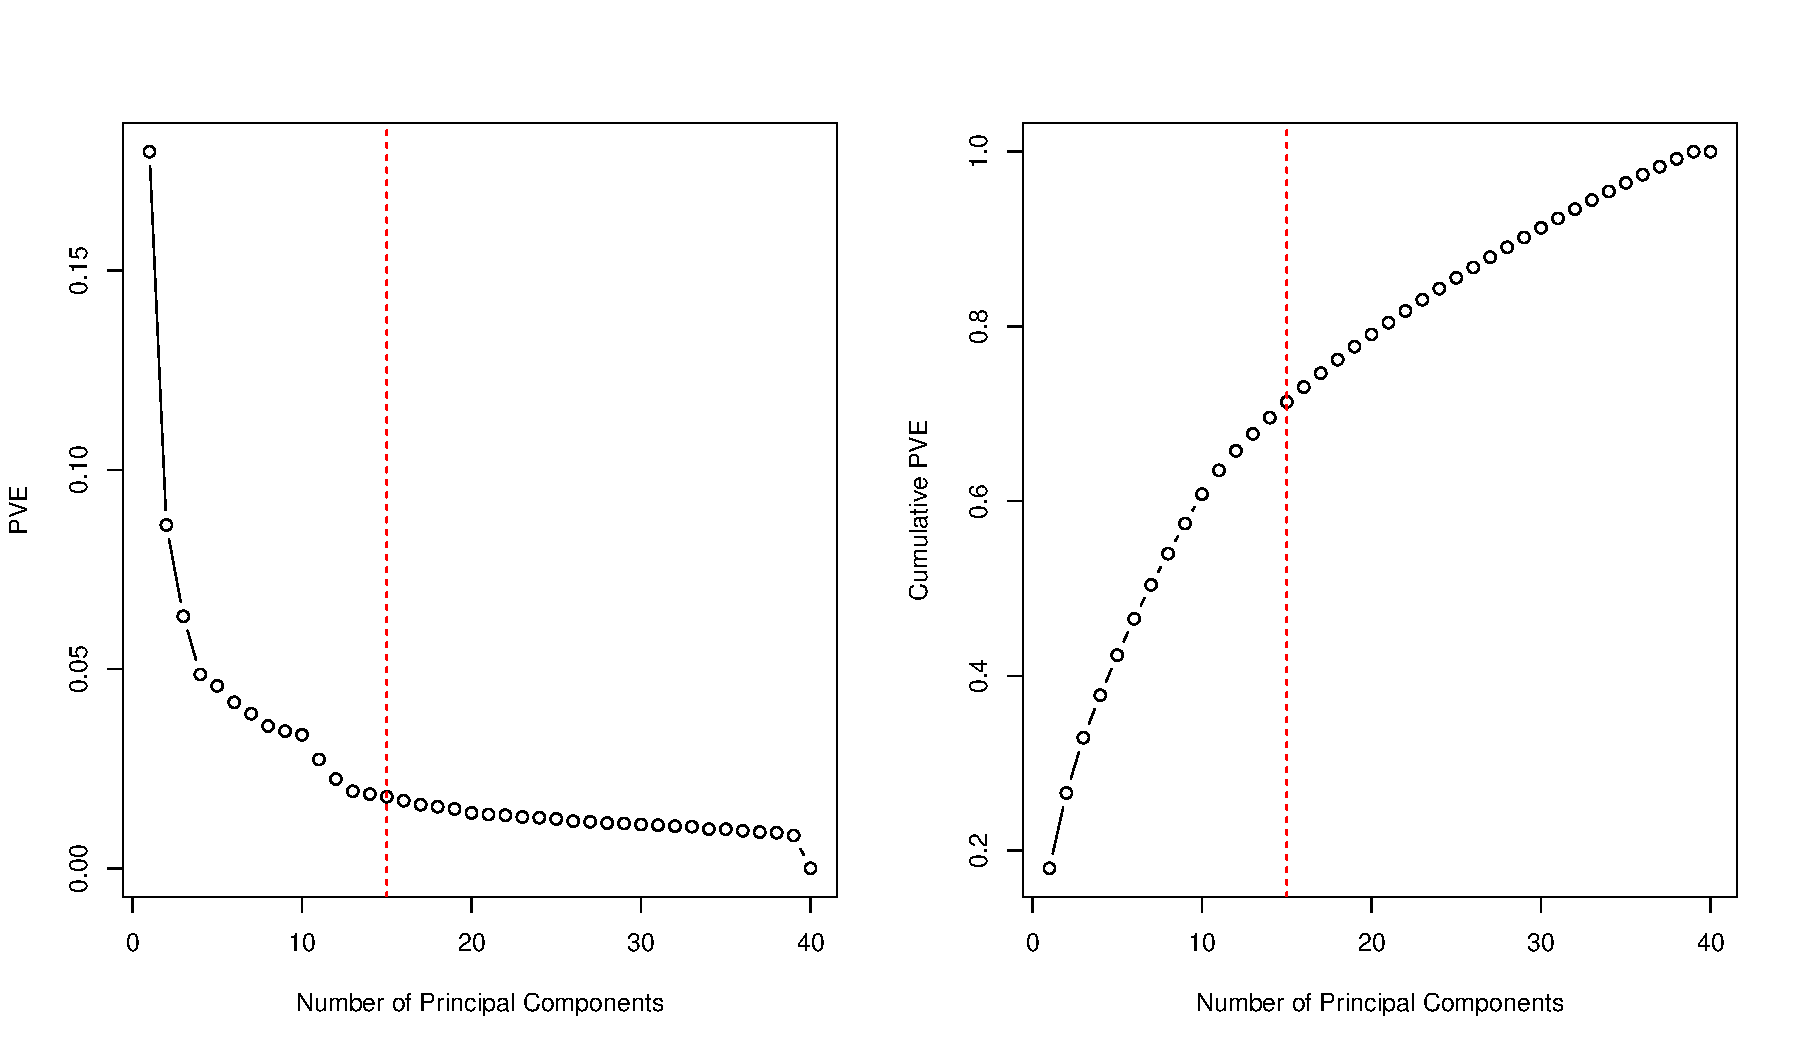
\includegraphics[width=\textwidth]{pca_dube_categ.pdf}
    \end{center}
  \end{figure}
\end{frame}

\begin{frame}{SVM}
  \begin{itemize}
    \item Optimised over three kernels; linear (SVC), polynomial and radial
      and respective parameters
      \begin{itemize}
        \item Linear: \texttt{cost}
        \item Polynomial: \texttt{cost}, \texttt{degree}
        \item Radial: \texttt{cost}, \texttt{gamma}
      \end{itemize}
    \item Linear (\texttt{cost} = 0.0785) and radial kernels gave (\texttt{cost}
      = 54.5559, \texttt{gamma} = 0.0034) best performance with 70\% accuracy
    \item Polynomial kernel (\texttt{cost} = 6.1585, \texttt{degree} = 1) lagged
      behind with 65\% accuracy
  \end{itemize} 
\end{frame}

\begin{frame}{KNN}
  \begin{itemize}
    \item Strong out-of-the-box classifier, \textit{nonparametric}
    \item Tends to suffer in high-dimensional settings
    \item Optimised for the number of nearest observations to inspect when
      classifying, \(K\) 
    \item \(K = 9\) gave the optimal accuracy of 75\%  \end{itemize}
\end{frame}

\begin{frame}{KNN}
  \begin{figure}
    \begin{center}
      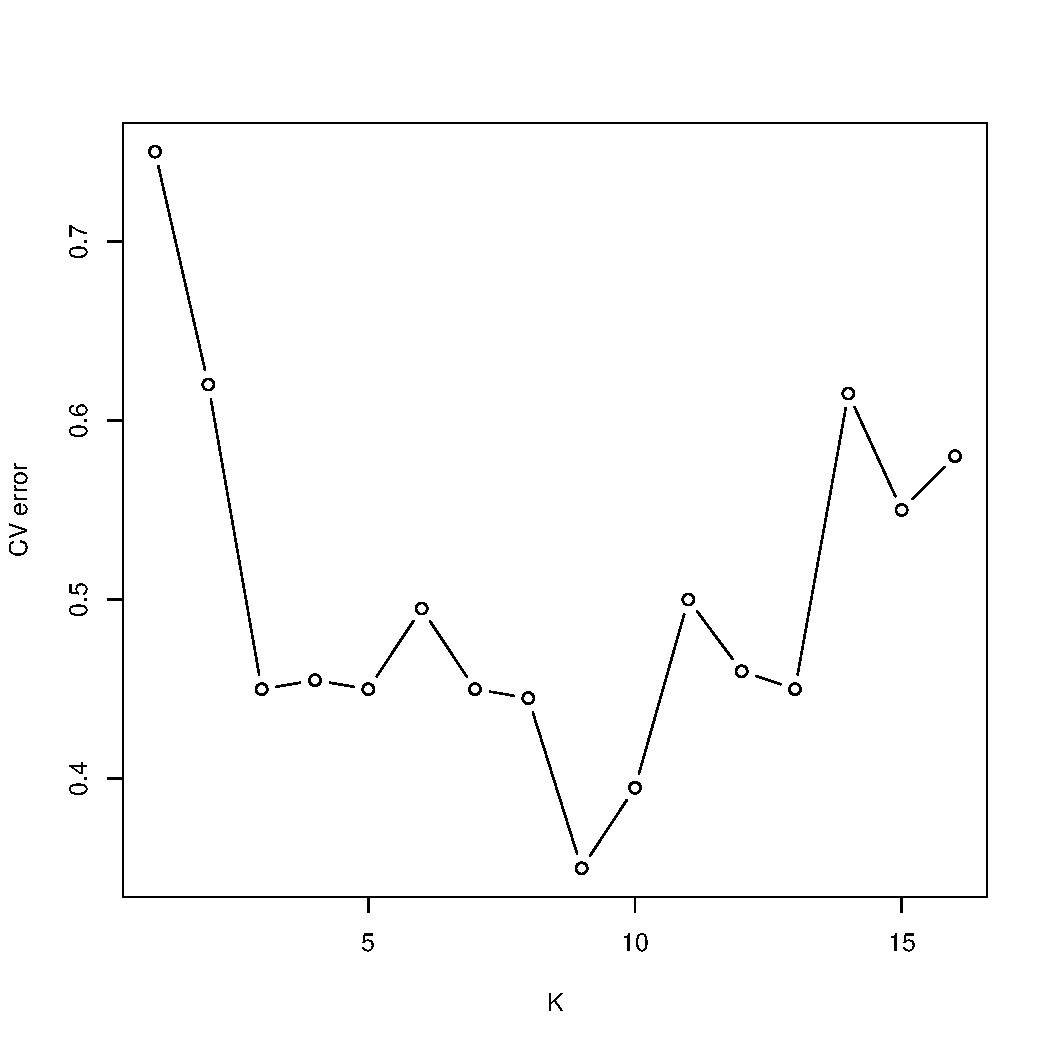
\includegraphics[width=0.7\textwidth]{knn_tuning.pdf}
    \end{center}
  \end{figure}
\end{frame}

\end{document}
